%%=============================================
% !Mode:: "TeX:UTF-8"
% !TEX program  = XeLaTeX
%%=============================================
% 模板名称:hitszthesis
% 模板版本:V3.0.3
% 模板作者:杨敬轩(Jingxuan Yang)
% 联系作者:yangjingxuan@stu.hit.edu.cn & yanglatex2e@gmail.com
% 模板交流:QQ群:1039392552,加群请备注LaTeX、hitszthesis相关说明
% 模板适用:哈尔滨工业大学(深圳)本、硕、博学位论文
% 模板编译:手动编译方法参看 README.md 或 hitszthesis.pdf
%          GNU make 工具:make thesis
%          Windows批处理脚本:双击 compile.bat 自动编译论文
%          更多编译细节详见说明文档:hitszthesis.pdf
% 更新时间:2020/03/12
% 模板帮助:请**务必务必务必**阅读 hitszthesis.pdf 说明文档,文档查看方法:
%          cmd 命令行:texdoc hitszthesis
%          推荐前往模板的 GitHub 仓库获取最新文件,地址:
%          https://github.com/YangLaTeX/hitszthesis
%%=============================================

% 设置文档类别为 <hitszthesis>,本文档为硕士学位论文示例
\documentclass[type=master]{hitszthesis}

% 模板提供以下选项,各个选项之间不要有空格
% 1. type=bachelor|master|doctor
%   含义:本科、硕士、博士学位论文,不设默认值,**必填**
% 2. covertitletworow=true|false
%   含义:本科封面第一页标题单行或多行显示,默认为单行显示(false)
% 3. infoleft=true|false
%   含义:本科封面第二页下划线内容居中或居左显示,默认为居中显示(false)
% 4. mathfont=newtxmath|mtprotwolite|mtprotwo
%   含义:正文数学字体选项:newtxmath(默认),mtprotwolite(lite版,免费),
%         mtprotwo(完全版,需购买授权),
%         mtpro2字体官网:https://www.pctex.com/mtpro2.html
% 5. boldcaption=true|false
%   含义:图表题注是否加粗,默认为不加粗(false)
% 6. tocfour=true|false
%   含义:是否添加第四级目录,只对本科文科个别要求四级目录有效,默认不添加(false)
% 7. fulltime=true|false
%   含义:是否全日制,非全日制如同等学力等,要在coverinformation中设置类型,
%        默认是全日制(true)
% 8. subtitle=true|false
%   含义:论文题目是否含有副标题,默认没有副标题(false)
% 9. openright=true|false
%   含义:博士论文是否要求章节首页必须在奇数页,默认否(false)
% 10. library=true|false
%   含义:是否为提交到图书馆的电子版,默认否(false)

% 自定义设置与额外加载的宏包请写在 \file{hitszthesis.sty} 里
\usepackage{hitszthesis}

% 图片存放路径,在这些文件夹里的图片可以直接使用图片文件名调用
\graphicspath{{figures/}{pictures/}}

%%=============================================
% 开始写论文
% !!注意本文仅作为排版格式示例,并不作为毕业论文规范
\begin{document}

% 若题目过长,则需使用以下命令调整本科封面第二页下划线长度
%\infowidth = 9cm

% 开始写前言部分
\frontmatter

% 封面信息填写
% !TEX root = ../main.tex

\hitszsetup{
  %******************************
  % 注意:
  %   1. 配置里面不要出现空行
  %   2. 不需要的配置信息可以删除
  %******************************
  %
  %=====
  % 秘级
  %=====
  statesecrets={公开},
  natclassifiedindex={TM301.2},
  intclassifiedindex={62-5},
  %
  %=========
  % 中文信息
  %=========
  ctitleone={基于神经网络的机器人},%本科生封面使用
  ctitletwo={智能抓取研究},%本科生封面使用
  ctitlecover={基于神经网络的机器人智能抓取研究},%放在封面中使用,自由断行
  ctitle={基于神经网络的机器人智能抓取研究},%放在原创性声明中使用
  csubtitle={一条副标题}, %一般情况没有,可以注释掉
  cxueke={工学},
  % csubject={机械设计制造及其自动化},
  csubject={机械工程},
  % caffil={机电工程与自动化学院},
  caffil={哈尔滨工业大学(深圳)},
  cauthor={杨敬轩},
  csupervisor={某某某 教授},
  cassosupervisor={某某某 教授}, % 副指导老师
  % ccosupervisor={某某某 教授}, % 联合指导老师
  % 日期自动使用当前时间,若需指定按如下方式修改:
  %cdate={超新星纪元},
  cstudentid={SZ160310217},
  cstudenttype={同等学力人员}, %非全日制教育申请学位者
  %(同等学力人员)、(工程硕士)、(工商管理硕士)、
  %(高级管理人员工商管理硕士)、(公共管理硕士)、(中职教师)、(高校教师)等
  %
  %
  %=========
  % 英文信息
  %=========
  etitle={Research on robot intelligent grasping based on Neural Network},
  esubtitle={This is the sub title},
  exueke={Engineering},
  esubject={Mechanical Engineering},
  eaffil={Harbin Institute of Technology, Shenzhen},
  eauthor={Jingxuan Yang},
  esupervisor={Prof. XXX},
  % eassosupervisor={XXX},
  % 日期自动生成,若需指定按如下方式修改:
  edate={June, 2020},
  estudenttype={Master of Engineering},
  %
  % 关键词用“英文逗号”分割
  ckeywords={\TeX, \LaTeX, CJK, 论文模板, 毕业论文},
  ekeywords={\TeX, \LaTeX, CJK, hitszthesis, thesis},
}

% 中文摘要
\begin{cabstract}

  摘要是论文内容的高度概括,应具有独立性和自含性,即不阅读论文的全文,就能获得必要的信息。摘要应包括本论文的目的、主要研究内容、研究方法、创造性成果及其理论与实际意义。摘要中不宜使用公式、化学结构式、图表和非公知公用的符号与术语,不标注引用文献编号,同时避免将摘要写成目录式的内容介绍。

  关键词是为了文献标引工作、用以表示全文主要内容信息的单词或术语。关键词不超过5个,每个关键词中间用分号分隔。(模板作者注:关键词分隔符不用考虑,模板会自动处理。英文关键词同理。)

\end{cabstract}

% 英文摘要
\begin{eabstract}

  Externally pressurized gas bearing has been widely used in the field of aviation, semiconductor, weave, and measurement apparatus because of its advantage of high accuracy, little friction, low heat distortion, long life-span, and no pollution. In this thesis, based on the domestic and overseas researching\dots\dots

  Key words are terms used in a dissertation for indexing, reflecting core information of the dissertation. An abstract may contain a maximum of 5 key words, with semi-colons used in between to separate one another.

\end{eabstract}


% 生成封面、中英文摘要
\makecover

% 物理量名称表,若采用标准符号则不需要此表
% % !TEX root = ../main.tex

% 物理量符号表,如果采用标准符号则不需要此表
\begin{denotation}
  % 此处最好是h
  \begin{table}[h]
  \caption{国际单位制中具有专门名称的导出单位}
  \vspace{0.5em}\centering\wuhao
  \begin{tabular}{ccccc}
    \toprule[1.5pt]
    量的名称&单位名称&单位符号&其它表示实例\\
    \midrule[1pt]
    频率&赫[兹]&Hz&s-1\\
    \bottomrule[1.5pt]
    \end{tabular}
  \end{table}
\end{denotation}


% 中文目录
\tableofcontents

% 开始写正文
\mainmatter

% 第1章
% !TEX root = ../main.tex

\chapter{绪论}

\section{课题背景及研究的目的和意义}

% 正文内容,注意LaTeX分段有两种方法,直接空一行或者使用<\par>
% 默认首行缩进,不需要在代码编辑区手动敲空格
发展国防工业、微电子工业等尖端技术需要精密和超精密的仪器设备,精密仪器设备要求高速、\dots\dots

\dots\dots

\section{气体润滑轴承及其相关理论的发展概况}

气体轴承是利用气膜支撑负荷或减少摩擦的机械构件。\dots\dots

\dots\dots

\subsection{气体润滑轴承的发展}

1828年,R.R.Willis$^{[3]}$发表了一篇关于小孔节流平板中压力分布的文章,这是有记载的研究气体润滑的最早文献。\dots\dots

根据间隙内气膜压力的产生原理,气体轴承可以分为四种基本形式:

(1)气体静压轴承:加压气体经过节流器进入间隙,在间隙内产生压力气膜使物体浮起的气体轴承,\dots\dots

\subsubsection{气体润滑轴承的分类}

\dots\dots

\subsubsection{多孔质气体静压轴承的研究}

由于气体的压力低和可压缩性,\dots\dots。

\section{本文的主要研究内容}

本课题的研究内容主要是针对局部多孔质止推轴承的多孔质材料的渗透
率、静压轴承的静态特性、稳定性及其影响因素进行展开,\dots\dots。


% 第2章
% !TEX root = ../main.tex

\chapter{排版图片}

\section{引言}
图应有自明性。插图应与文字紧密配合,文图相符,内容正确。选图要力求精练,插图、照
片应完整清晰。

\section{运动学分析}

考虑三个空间,分别是驱动空间、关节空间以及操作空间。驱动空间包含的是各个绳索长度组成的矩阵,不同时刻绳索长度可能不同。关节空间包含的是机械臂各个关节的关节角组成的矩阵,不同时刻关节角可能不同。操作空间包含的是机械臂末端位姿组成的位姿矩阵,不同时刻位姿可能不同,单个关节三维模型如\figref{fig:bm}所示。

\begin{figure}[ht]
\centering
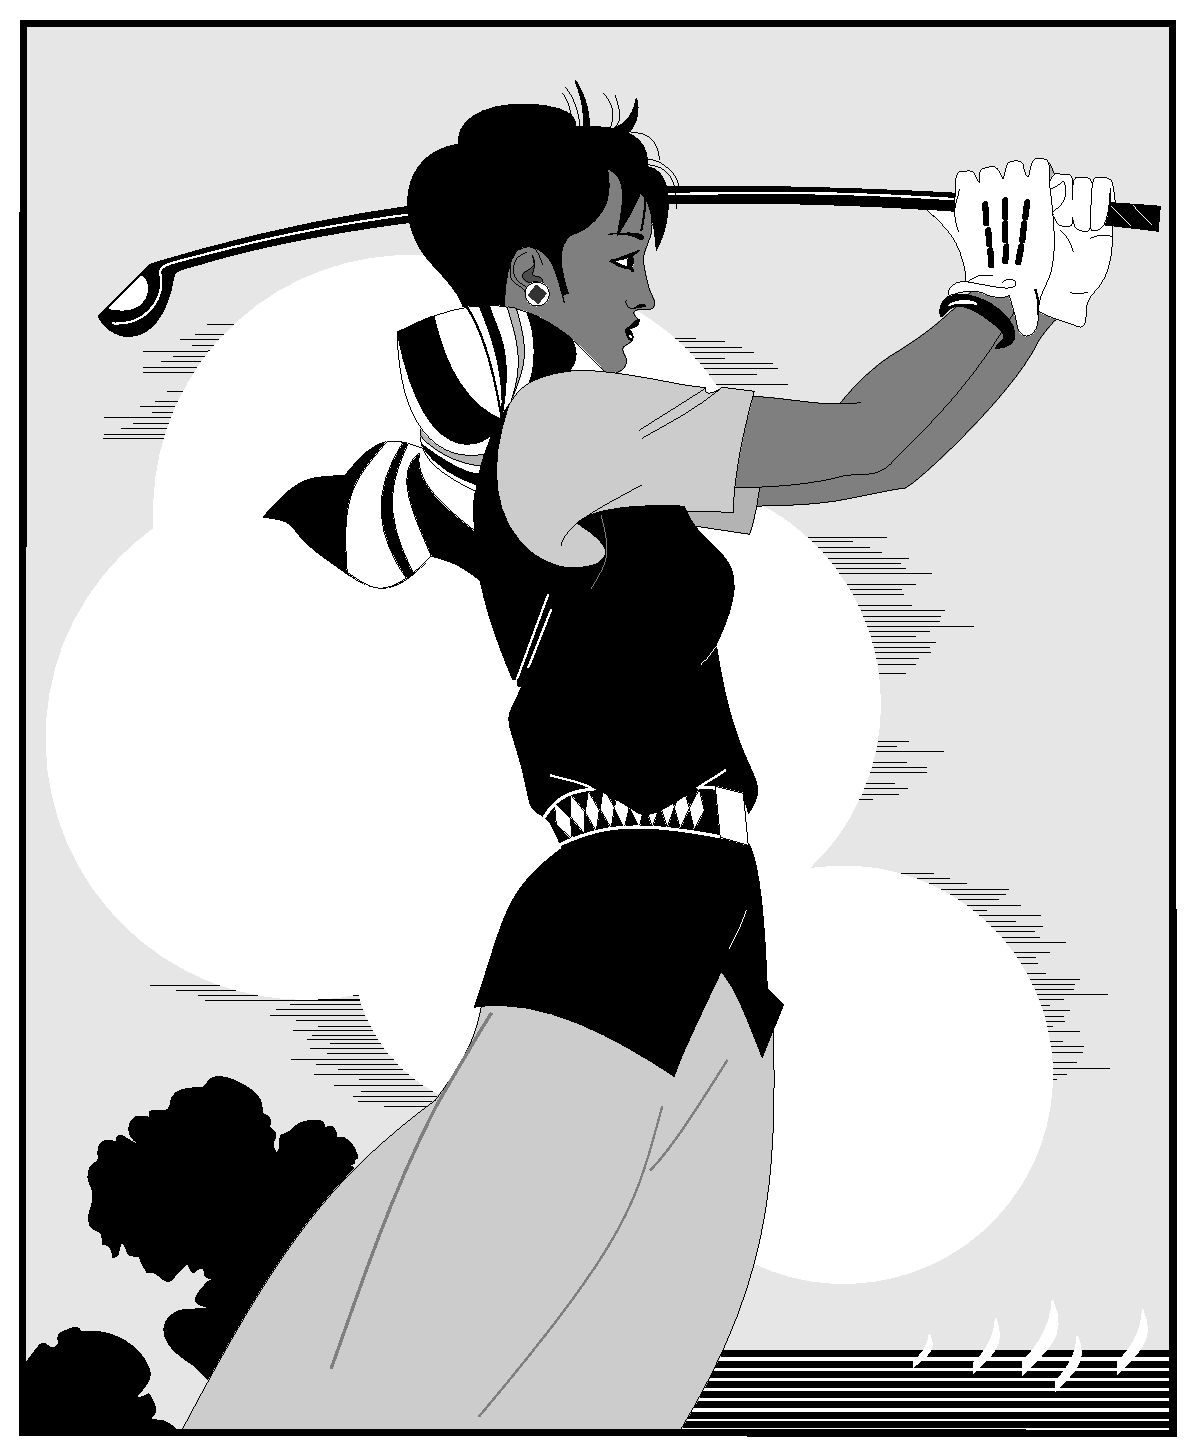
\includegraphics[width = 0.4\textwidth]{golfer}
\caption{打高尔夫球的人}
\label{fig:bm}
\end{figure}

\subsection{内容XXX}

\lipsum[3]

\section{内容XXX}

\lipsum[2]

\section{本章小结}

\lipsum[1]


% 第3章
% !TEX root = ../main.tex

\chapter{内容XXX}

\section{引言}

每章的引言起到承接上一章引启下一章的作用。

\ldots\ldots

\section{对物理量符号进行注释的情况}

为使得对公式中物理量符号注释的转行与破折号“———”后第一个字对齐,此处最好采用表格环境。此表格无任何线条,左对齐,且在破折号处对齐,一共有“式中”二字、物理量符号和注释三列,表格的总宽度可选为文本宽度,因此应该采用\verb|tabularx|环境。由\verb|tabularx|环境生成的对公式中物理量符号进行注释的公式如式(\ref{eq:1})所示。
\begin{equation}\label{eq:1}
\ddot{\bm{\rho}}-\frac{\mu}{R_{t}^{3}}\left(3\bm{R_{t}}\frac{\bm{R_{t}\rho}}{R_{t}^{2}}-\bm{\rho}\right)=\bm{a}
\end{equation}
\begin{tabularx}{\textwidth}{@{}l@{\quad}r@{———}X@{}}
式中& $\bm{\rho}$ &追踪飞行器与目标飞行器之间的相对位置矢量;\\
&  $\bm{\ddot{\rho}}$&追踪飞行器与目标飞行器之间的相对加速度;\\
&  $\bm{a}$   &推力所产生的加速度;\\
&  $\bm{R_t}$ & 目标飞行器在惯性坐标系中的位置矢量;\\
&  $\omega_{t}$ & 目标飞行器的轨道角速度;\\
\end{tabularx}\vspace{3.15bp}
由此方法生成的注释内容应紧邻待注释公式并置于其下方,因此不能将代码放入\verb|table|浮动环境中。但此方法不能实现自动转页接排,可能会在当前页剩余空间不够时,全部移动到下一页而导致当前页出现很大空白。因此在需要转页处理时,还请您手动将需要转页的代码放入一个新的\verb|tabularx|环境中,将原来的一个\verb|tabularx|环境拆分为两个\verb|tabularx|环境。

{\color{red}(矩阵、矢量用“粗、斜体”,如矢量$\bm{R}$;单变量用“斜体”(不加粗),如$x,y$;上下标:有变量含义的用斜体,如$x_i$;数字、单词首字母、单位等无变量含义的用正体,如$x_1$,矩阵转置$\bm{A}^{\text{T}}$(T 为转置Transpose 的首字母))}

\section{子公式}

子公式编号示例:如果需要对公式的子公式进行编号,则使用\lstinline{subeqnarray}环境:
\begin{subeqnarray}
  \label{eqw}
  \slabel{eq0}
  x & = & a \times b \\
  \slabel{eq1}
  & = & z + t\\
  \slabel{eq2}
  & = & z + t
\end{subeqnarray}

\equref{eqw}中,\lstinline{label}为整个公式的标签,\lstinline{slabel}为子公式的标签。

\section{本章小结}

总结本章的叙述内容。

\lipsum[1]


% 第4章
% !TEX root = ../main.tex

\chapter{内容XXX}

\section{引言}

每章的引言起到承接上一章引启下一章的作用。

\ldots\ldots

\section{普通表格的绘制方法}

表格应具有三线表格式,因此需要调用~booktabs~宏包,其标准格式如表~\ref{table1}~所示。
\begin{table}[htbp]
\caption{符合研究生院绘图规范的表格}
\label{table1}
\vspace{0.5em}\centering\wuhao
\begin{tabular}{ccccc}
\toprule[1.5pt]
$D$(in) & $P_u$(lbs) & $u_u$(in) & $\beta$ & $G_f$(psi.in)\\
\midrule[1pt]
 5 & 269.8 & 0.000674 & 1.79 & 0.04089\\
10 & 421.0 & 0.001035 & 3.59 & 0.04089\\
20 & 640.2 & 0.001565 & 7.18 & 0.04089\\
\bottomrule[1.5pt]
\end{tabular}
\end{table}
全表如用同一单位,则将单位符号移至表头右上角,加圆括号。表中数据应准确无误,书写清楚。数字空缺的格内加横线“-”(占~2~个数字宽度)。表内文字或数字上、下或左、右相同时,采用通栏处理方式,不允许用“〃”、“同上”之类的写法。表内文字说明,起行空一格、转行顶格、句末不加标点。如某个表需要转页接排,在随后的各页上应重复表的编号。编号后加“(续表)”,表题可省略。续表应重复表头。

\section{XXXX分析}

\lipsum[1]

\section{XXXX分析}

\lipsum[2]

\section{本章小结}

总结本章的叙述内容。

\lipsum[3]


% 第5章
% !TEX root = ../main.tex

\chapter{内容XXX}

\section{引言}

每章的引言起到承接上一章引启下一章的作用。

\ldots\ldots

\section{参考文献引用方法}

\sindex[china]{du!段誉}引文标注遵照GB/T7714-2005,采用顺序编码制。正文中引用文献的标示应置于所引内容最后一个字的右上角,所引文献编号用阿拉伯数字置于方括号“[ ]”中,用小4号字体的上角标。要求:

(1)引用单篇文献时,如“二次铣削\cite{ren2010}”。

(2)同一处引用多篇文献时,各篇文献的序号在方括号内全部列出,各序号间用“,”,如
遇连续序号,可标注讫序号。如,…形成了多种数学模型\cite{Gravagne2003,ren2010}…
注意此处添加\cs{inlinecite}中文空格\inlinecite{Gravagne2003,ren2010},可以在cfg文件中修改空格类型。

(3)多次引用同一文献时,在文献序号的“[ ]”后标注引文页码。如,…间质细胞CAMP含量
测定\cite[100-197]{Gravagne2003}…。…含量测定方法规定
\cite[92]{Gravagne2003}…。

(4)当提及的参考文献为文中直接说明时,则用小4号字与正文排齐,如“由文献\inlinecite{webster2010}可知”

(5)多\cite{liu2016}引\cite{fu2018}用\cite{zhai2015}一\cite{yao2015}些\cite{jones2006}参\cite{mcmahan2005}考\cite{jones2004}文献以生成附录参考文献。

\section{XXXX分析}

\lipsum[1-2]

\section{本章小结}

总结本章的叙述内容。

\lipsum[1]


% 第6章
% !TEX root = ../main.tex

% 中英标题:\chapter{中文标题}[英文标题]
\chapter{补充说明}

\section{引言}

\lipsum[2]

\section{内容XXX}

\lipsum[3]

\section{内容XXX}

\lipsum[3]

\section{本章小结}

\lipsum[2]


% 开始写正文之后的部分
\backmatter

% 结论
% !TEX root = ../main.tex

% 结论
\begin{conclusions}

学位论文的结论作为论文正文的最后一章单独排写,但不加章标题序号。

结论应是作者在学位论文研究过程中所取得的创新性成果的概要总结,不能与摘要混为一谈。博士学位论文结论应包括论文的主要结果、创新点、展望三部分,在结论中应概括论文的核心观点,明确、客观地指出本研究内容的创新性成果(含新见解、新观点、方法创新、技术创新、理论创新),并指出今后进一步在本研究方向进行研究工作的展望与设想。对所取得的创新性成果应注意从定性和定量两方面给出科学、准确的评价,分(1)、(2)、(3)…条列出,宜用“提出了”、“建立了”等词叙述。

\end{conclusions}


% 参考文献
\bibliographystyle{hitszthesis}
\bibliography{reference}

% 附录
\begin{appendix}
  % !TEX root = ../main.tex

% 附录A
\chapter{带章节的附录}[Full Appendix]

完整的附录内容,包含章节,公式,图表等。

\section{附录节的内容}[Section in Appendix]

这是附录的节的内容。

附录中\figref{fig:appA}:
\begin{figure}[htbp]
\centering
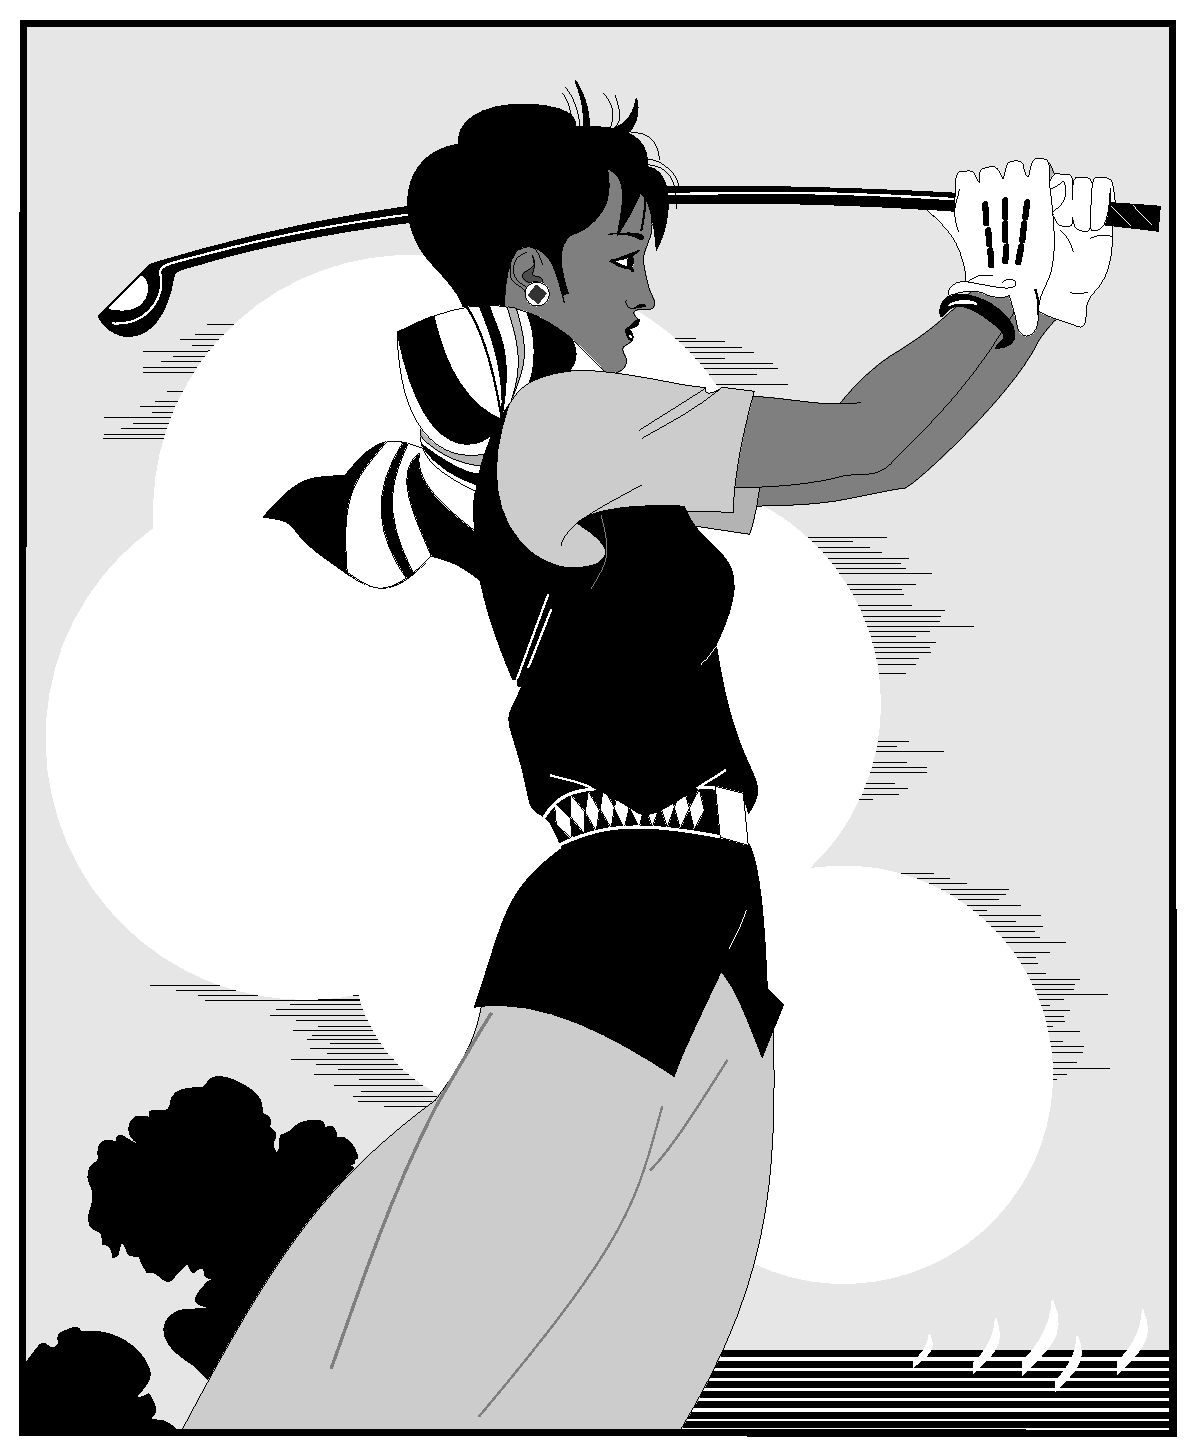
\includegraphics[width = 0.4\textwidth]{golfer}
%\bicaption[golfer5]{}{\xiaosi[0]打高尔夫球的人}{Fig.$\!$}{The person playing golf}\vspace{-1em}
\caption{\xiaosi[0]打高尔夫球的人}
\label{fig:appA}
\end{figure}

附录中\equref{eq:appA}:
\begin{align}
a & = b \times c \\
E & = m c^2
\label{eq:appA}
\end{align}

  % !TEX root = ../main.tex

% 附录B
\chapter{其他附录}[Other appendices]

其他附录内容可以放在这里。

\end{appendix}

% 发表文章
% !TEX root = ../main.tex

% 发表论文、专利、获奖情况
\begin{publication}
  \noindent\songti\textbf{(一)发表的学术论文}
  \begin{publist}
    \item	XXX,XXX. Static Oxidation Model of Al-Mg/C Dissipation Thermal Protection Materials[J]. Rare Metal Materials and Engineering, 2010, 39(Suppl. 1): 520-524.(SCI~收录,IDS号为~669JS,IF=0.16)
    \item XXX,XXX. 精密超声振动切削单晶铜的计算机仿真研究[J]. 系统仿真学报,2007,19(4):738-741,753.(EI~收录号:20071310514841)
    \item XXX,XXX. 局部多孔质气体静压轴向轴承静态特性的数值求解[J]. 摩擦学学报,2007(1):68-72.(EI~收录号:20071510544816)
    \item XXX,XXX. 硬脆光学晶体材料超精密切削理论研究综述[J]. 机械工程学报,2003,39(8):15-22.(EI~收录号:2004088028875)
    \item XXX,XXX. 基于遗传算法的超精密切削加工表面粗糙度预测模型的参数辨识以及切削参数优化[J]. 机械工程学报,2005,41(11):158-162.(EI~收录号:2006039650087)
    \item XXX,XXX. Discrete Sliding Mode Cintrok with Fuzzy Adaptive Reaching Law on 6-PEES Parallel Robot[C]. Intelligent System Design and Applications, Jinan, 2006: 649-652.(EI~收录号:20073210746529)
  \end{publist}

  \noindent\songti\textbf{(二)申请及已获得的专利(无专利时此项不必列出)}
  \begin{publist}
    \item XXX,XXX. 一种温热外敷药制备方案:中国,88105607.3[P]. 1989-07-26.
  \end{publist}

  \noindent\songti\textbf{(三)参与的科研项目及获奖情况}
  \begin{publist}
    \item	XXX,XXX. XX~气体静压轴承技术研究, XX~省自然科学基金项目.课题编号:XXXX.
    \item XXX,XXX. XX~静载下预应力混凝土房屋结构设计统一理论. 黑江省科学技术二等奖, 2007.
  \end{publist}
  %\vfill
  %\hangafter=1\hangindent=2em\noindent
  %\setlength{\parindent}{2em}
\end{publication}


% 授权
\authorization

% 授权页为扫描的PDF文件(scan.pdf),与上面的命令互斥
% \authorization[scan.pdf]

% 致谢
% !TEX root = ../main.tex

% 致谢
\begin{acknowledgements}

衷心感谢导师XXX教授对本人的精心指导。他的言传身教将使我终生受益。

感谢XXX教授,以及实验室全体老师和同窗们的热情帮助和支持!

本课题承蒙XXXX基金资助,特此致谢。

\ldots\ldots

\end{acknowledgements}


% 个人简介
% % !TEX root = ../main.tex

% 个人简历
\begin{resume}

  XXXX~年~XX~月~XX~日出生于~XXXX。

  XXXX~年~XX~月考入~XX~大学~XX~院(系)XX~专业,XXXX~年~XX~月本科毕业并获得~XX~学学士学位。

  XXXX~年~XX~月------XXXX~年~XX~月在~XX~大学~XX~院(系)XX~学科学习并获得~XX~学硕士学位。

  XXXX~年~XX~月------XXXX~年~XX~月在~XX~大学~XX~院(系)XX~学科学习并获得~XX~学博士学位。

  获奖情况:如获三好学生、优秀团干部、X~奖学金等(不含科研学术获奖)。

  工作经历:

  \songti\textbf{(除全日制硕士生以外,其余学生均应增列此项。个人简历一般应包含教育经历和工作经历。)}

\end{resume}


% 结束文档撰写
\end{document}
%%=============================================

% Local Variables:
% TeX-engine: xetex
% End:
